% Options for packages loaded elsewhere
\PassOptionsToPackage{unicode}{hyperref}
\PassOptionsToPackage{hyphens}{url}
\PassOptionsToPackage{dvipsnames,svgnames,x11names}{xcolor}
%
\documentclass[
  letterpaper,
  DIV=11,
  numbers=noendperiod]{scrartcl}

\usepackage{amsmath,amssymb}
\usepackage{lmodern}
\usepackage{iftex}
\ifPDFTeX
  \usepackage[T1]{fontenc}
  \usepackage[utf8]{inputenc}
  \usepackage{textcomp} % provide euro and other symbols
\else % if luatex or xetex
  \usepackage{unicode-math}
  \defaultfontfeatures{Scale=MatchLowercase}
  \defaultfontfeatures[\rmfamily]{Ligatures=TeX,Scale=1}
\fi
% Use upquote if available, for straight quotes in verbatim environments
\IfFileExists{upquote.sty}{\usepackage{upquote}}{}
\IfFileExists{microtype.sty}{% use microtype if available
  \usepackage[]{microtype}
  \UseMicrotypeSet[protrusion]{basicmath} % disable protrusion for tt fonts
}{}
\makeatletter
\@ifundefined{KOMAClassName}{% if non-KOMA class
  \IfFileExists{parskip.sty}{%
    \usepackage{parskip}
  }{% else
    \setlength{\parindent}{0pt}
    \setlength{\parskip}{6pt plus 2pt minus 1pt}}
}{% if KOMA class
  \KOMAoptions{parskip=half}}
\makeatother
\usepackage{xcolor}
\setlength{\emergencystretch}{3em} % prevent overfull lines
\setcounter{secnumdepth}{-\maxdimen} % remove section numbering
% Make \paragraph and \subparagraph free-standing
\ifx\paragraph\undefined\else
  \let\oldparagraph\paragraph
  \renewcommand{\paragraph}[1]{\oldparagraph{#1}\mbox{}}
\fi
\ifx\subparagraph\undefined\else
  \let\oldsubparagraph\subparagraph
  \renewcommand{\subparagraph}[1]{\oldsubparagraph{#1}\mbox{}}
\fi

\usepackage{color}
\usepackage{fancyvrb}
\newcommand{\VerbBar}{|}
\newcommand{\VERB}{\Verb[commandchars=\\\{\}]}
\DefineVerbatimEnvironment{Highlighting}{Verbatim}{commandchars=\\\{\}}
% Add ',fontsize=\small' for more characters per line
\usepackage{framed}
\definecolor{shadecolor}{RGB}{241,243,245}
\newenvironment{Shaded}{\begin{snugshade}}{\end{snugshade}}
\newcommand{\AlertTok}[1]{\textcolor[rgb]{0.68,0.00,0.00}{#1}}
\newcommand{\AnnotationTok}[1]{\textcolor[rgb]{0.37,0.37,0.37}{#1}}
\newcommand{\AttributeTok}[1]{\textcolor[rgb]{0.40,0.45,0.13}{#1}}
\newcommand{\BaseNTok}[1]{\textcolor[rgb]{0.68,0.00,0.00}{#1}}
\newcommand{\BuiltInTok}[1]{\textcolor[rgb]{0.00,0.23,0.31}{#1}}
\newcommand{\CharTok}[1]{\textcolor[rgb]{0.13,0.47,0.30}{#1}}
\newcommand{\CommentTok}[1]{\textcolor[rgb]{0.37,0.37,0.37}{#1}}
\newcommand{\CommentVarTok}[1]{\textcolor[rgb]{0.37,0.37,0.37}{\textit{#1}}}
\newcommand{\ConstantTok}[1]{\textcolor[rgb]{0.56,0.35,0.01}{#1}}
\newcommand{\ControlFlowTok}[1]{\textcolor[rgb]{0.00,0.23,0.31}{#1}}
\newcommand{\DataTypeTok}[1]{\textcolor[rgb]{0.68,0.00,0.00}{#1}}
\newcommand{\DecValTok}[1]{\textcolor[rgb]{0.68,0.00,0.00}{#1}}
\newcommand{\DocumentationTok}[1]{\textcolor[rgb]{0.37,0.37,0.37}{\textit{#1}}}
\newcommand{\ErrorTok}[1]{\textcolor[rgb]{0.68,0.00,0.00}{#1}}
\newcommand{\ExtensionTok}[1]{\textcolor[rgb]{0.00,0.23,0.31}{#1}}
\newcommand{\FloatTok}[1]{\textcolor[rgb]{0.68,0.00,0.00}{#1}}
\newcommand{\FunctionTok}[1]{\textcolor[rgb]{0.28,0.35,0.67}{#1}}
\newcommand{\ImportTok}[1]{\textcolor[rgb]{0.00,0.46,0.62}{#1}}
\newcommand{\InformationTok}[1]{\textcolor[rgb]{0.37,0.37,0.37}{#1}}
\newcommand{\KeywordTok}[1]{\textcolor[rgb]{0.00,0.23,0.31}{#1}}
\newcommand{\NormalTok}[1]{\textcolor[rgb]{0.00,0.23,0.31}{#1}}
\newcommand{\OperatorTok}[1]{\textcolor[rgb]{0.37,0.37,0.37}{#1}}
\newcommand{\OtherTok}[1]{\textcolor[rgb]{0.00,0.23,0.31}{#1}}
\newcommand{\PreprocessorTok}[1]{\textcolor[rgb]{0.68,0.00,0.00}{#1}}
\newcommand{\RegionMarkerTok}[1]{\textcolor[rgb]{0.00,0.23,0.31}{#1}}
\newcommand{\SpecialCharTok}[1]{\textcolor[rgb]{0.37,0.37,0.37}{#1}}
\newcommand{\SpecialStringTok}[1]{\textcolor[rgb]{0.13,0.47,0.30}{#1}}
\newcommand{\StringTok}[1]{\textcolor[rgb]{0.13,0.47,0.30}{#1}}
\newcommand{\VariableTok}[1]{\textcolor[rgb]{0.07,0.07,0.07}{#1}}
\newcommand{\VerbatimStringTok}[1]{\textcolor[rgb]{0.13,0.47,0.30}{#1}}
\newcommand{\WarningTok}[1]{\textcolor[rgb]{0.37,0.37,0.37}{\textit{#1}}}

\providecommand{\tightlist}{%
  \setlength{\itemsep}{0pt}\setlength{\parskip}{0pt}}\usepackage{longtable,booktabs,array}
\usepackage{calc} % for calculating minipage widths
% Correct order of tables after \paragraph or \subparagraph
\usepackage{etoolbox}
\makeatletter
\patchcmd\longtable{\par}{\if@noskipsec\mbox{}\fi\par}{}{}
\makeatother
% Allow footnotes in longtable head/foot
\IfFileExists{footnotehyper.sty}{\usepackage{footnotehyper}}{\usepackage{footnote}}
\makesavenoteenv{longtable}
\usepackage{graphicx}
\makeatletter
\def\maxwidth{\ifdim\Gin@nat@width>\linewidth\linewidth\else\Gin@nat@width\fi}
\def\maxheight{\ifdim\Gin@nat@height>\textheight\textheight\else\Gin@nat@height\fi}
\makeatother
% Scale images if necessary, so that they will not overflow the page
% margins by default, and it is still possible to overwrite the defaults
% using explicit options in \includegraphics[width, height, ...]{}
\setkeys{Gin}{width=\maxwidth,height=\maxheight,keepaspectratio}
% Set default figure placement to htbp
\makeatletter
\def\fps@figure{htbp}
\makeatother
\newlength{\cslhangindent}
\setlength{\cslhangindent}{1.5em}
\newlength{\csllabelwidth}
\setlength{\csllabelwidth}{3em}
\newlength{\cslentryspacingunit} % times entry-spacing
\setlength{\cslentryspacingunit}{\parskip}
\newenvironment{CSLReferences}[2] % #1 hanging-ident, #2 entry spacing
 {% don't indent paragraphs
  \setlength{\parindent}{0pt}
  % turn on hanging indent if param 1 is 1
  \ifodd #1
  \let\oldpar\par
  \def\par{\hangindent=\cslhangindent\oldpar}
  \fi
  % set entry spacing
  \setlength{\parskip}{#2\cslentryspacingunit}
 }%
 {}
\usepackage{calc}
\newcommand{\CSLBlock}[1]{#1\hfill\break}
\newcommand{\CSLLeftMargin}[1]{\parbox[t]{\csllabelwidth}{#1}}
\newcommand{\CSLRightInline}[1]{\parbox[t]{\linewidth - \csllabelwidth}{#1}\break}
\newcommand{\CSLIndent}[1]{\hspace{\cslhangindent}#1}

\KOMAoption{captions}{tableheading}
\makeatletter
\makeatother
\makeatletter
\makeatother
\makeatletter
\@ifpackageloaded{caption}{}{\usepackage{caption}}
\AtBeginDocument{%
\ifdefined\contentsname
  \renewcommand*\contentsname{Table of contents}
\else
  \newcommand\contentsname{Table of contents}
\fi
\ifdefined\listfigurename
  \renewcommand*\listfigurename{List of Figures}
\else
  \newcommand\listfigurename{List of Figures}
\fi
\ifdefined\listtablename
  \renewcommand*\listtablename{List of Tables}
\else
  \newcommand\listtablename{List of Tables}
\fi
\ifdefined\figurename
  \renewcommand*\figurename{Figure}
\else
  \newcommand\figurename{Figure}
\fi
\ifdefined\tablename
  \renewcommand*\tablename{Table}
\else
  \newcommand\tablename{Table}
\fi
}
\@ifpackageloaded{float}{}{\usepackage{float}}
\floatstyle{ruled}
\@ifundefined{c@chapter}{\newfloat{codelisting}{h}{lop}}{\newfloat{codelisting}{h}{lop}[chapter]}
\floatname{codelisting}{Listing}
\newcommand*\listoflistings{\listof{codelisting}{List of Listings}}
\makeatother
\makeatletter
\@ifpackageloaded{caption}{}{\usepackage{caption}}
\@ifpackageloaded{subcaption}{}{\usepackage{subcaption}}
\makeatother
\makeatletter
\@ifpackageloaded{tcolorbox}{}{\usepackage[many]{tcolorbox}}
\makeatother
\makeatletter
\@ifundefined{shadecolor}{\definecolor{shadecolor}{rgb}{.97, .97, .97}}
\makeatother
\makeatletter
\makeatother
\ifLuaTeX
  \usepackage{selnolig}  % disable illegal ligatures
\fi
\IfFileExists{bookmark.sty}{\usepackage{bookmark}}{\usepackage{hyperref}}
\IfFileExists{xurl.sty}{\usepackage{xurl}}{} % add URL line breaks if available
\urlstyle{same} % disable monospaced font for URLs
\hypersetup{
  pdftitle={Group 34 course work},
  colorlinks=true,
  linkcolor={blue},
  filecolor={Maroon},
  citecolor={Blue},
  urlcolor={Blue},
  pdfcreator={LaTeX via pandoc}}

\title{Group 34 course work}
\author{}
\date{}

\begin{document}
\maketitle
\ifdefined\Shaded\renewenvironment{Shaded}{\begin{tcolorbox}[borderline west={3pt}{0pt}{shadecolor}, enhanced, frame hidden, boxrule=0pt, breakable, interior hidden, sharp corners]}{\end{tcolorbox}}\fi

\renewcommand*\contentsname{Table of contents}
{
\hypersetup{linkcolor=}
\setcounter{tocdepth}{3}
\tableofcontents
}
\hypertarget{force-a-page-break-here}{%
\subsection{FOrce a page break here}\label{force-a-page-break-here}}

\hypertarget{introduction}{%
\subsection{Introduction:}\label{introduction}}

Tuberculosis (TB) is a bacterial disease caused by the bacterium
Mycobacterium tuberculosis. It primarily affects the lungs, but can also
affect other parts of the body, such as the kidneys, spine, and brain.

TB is a major public health problem worldwide, affecting millions of
people each year. According to the World Health Organization (WHO), TB
is one of the top 10 causes of death worldwide, and in 2020 alone, there
were an estimated of approximately 10 million cases of TB reported
globally. Brazil is one of the countries with a high burden of TB with
an estimate of 96000, and it is considered a priority country for TB
control by the WHO. \emph{Global Tuberculosis Report 2020} (2020).

The purpose of this report is to provide a comprehensive analysis of TB
in Brazil from the 2012 to 2014 data, including an overview of the
trends and risk factors associated with TB. Additionally, this report
aims to highlight the most important factor for improving TB control and
prevention efforts in Brazil.

The case study we will consider in this report is the Tuberculosis
dataframe where Brazil is divided into 557 administrative microregions
and the available data comprises of counts of TB cases in each
microregion from 2012 to 2014.

\hypertarget{exploratory-data-analysis}{%
\subsection{Exploratory Data
Analysis:}\label{exploratory-data-analysis}}

\begin{verbatim}
<!-- Provide a summary of the Tuberculosis dataset, including descriptive statistics and visualizations. -->
<!-- Identify any patterns or trends in the data, such as geographical or temporal clusters of cases. -->
<!-- Discuss any issues with the data, such as outliers or inconsistencies. -->
\end{verbatim}

The TBdata dataframe contains information on various socio-demographic
and geographic factors in Brazil that may be associated with TB
incidence in each microregion. These factors include indigenous
population, illiteracy levels, urbanization rate, dwelling density,
poverty levels, sanitation levels, unemployment rates, and timeliness of
TB case reporting. The dataset also includes information on the number
of TB cases and population size for each microregion, as well as unique
ID numbers to distinguish between the different regions.

An exploratory analysis of this dataset can reveal important insights of
the potential risk factors for TB in Brazil and help guide public health
interventions.

We will start by analysing the distributions of each of the variables to
identify any patterns 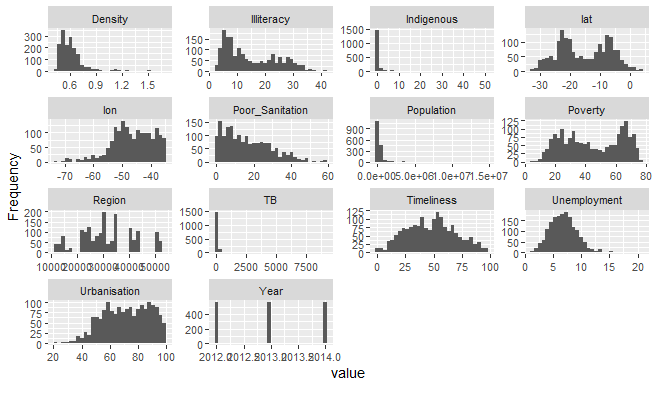
\includegraphics{histogramExploratoryAnalysis.png}

Firstly, the dwelling density seems to follow a normal distribution that
is skewed to the right and a mean of approximately 0,6.

Secondly illiteracy is very heavily skewed to the right but it still
displays a normal bell curve around the 5\% illiteracy level.

Poor sanitation is

Unemployment seems to follow a normal distribution with little to no
skewness and a mean of approximately 6\%.

\begin{figure}

{\centering 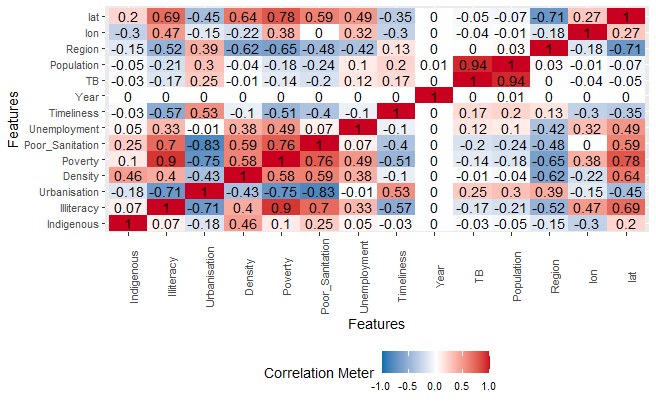
\includegraphics{HeatMap.png}

}

\caption{Correlation Matrix}

\end{figure}

As we can see from the matrix, the variable that is the most correlated
from TB is the population, with illiteracy, poor sanitation and poverty
having a negative correlation with TB.

\hypertarget{model-selection}{%
\subsection{Model Selection:}\label{model-selection}}

We are utilising generalized additive models (GAMs) in the case study of
TB in Brazil as it can model complex and nonlinear relationships between
TB incidence and risk factors, control for relevant covariates, identify
important predictors of TB incidence, and predict TB incidence in
different regions of Brazil.

As the data is count data we will first fit a Poisson module since this
distribution is a good fit for the nature of the data

Yi ∼ Pois(\(\lambda\)) Yi indep.

Log(\(\lambda i\)) =
\(offset(log(Populationi))+fIndigenous(Indigenousi)+fIlliteracy(Illiteracyi)+fUrbanisation(Urbanisationi)+fDensity(Densityi)+fPoverty(Povertyi)+fPoor_Sanitation(Poor_Sanitationi)+fUnemployment(Unemploymenti)+fTimeliness(Timelinessi)+fla(lati)+flon(loni)+fYear(Yeari)+flon,lat,Year(loni,lati,Yeari)\)

However the Poisson model seems to not have a good enough fitting
results and as such we will extend the model into a negative binomial
GAM

\hypertarget{model-fitting}{%
\subsection{Model Fitting:}\label{model-fitting}}

\begin{figure}

{\centering 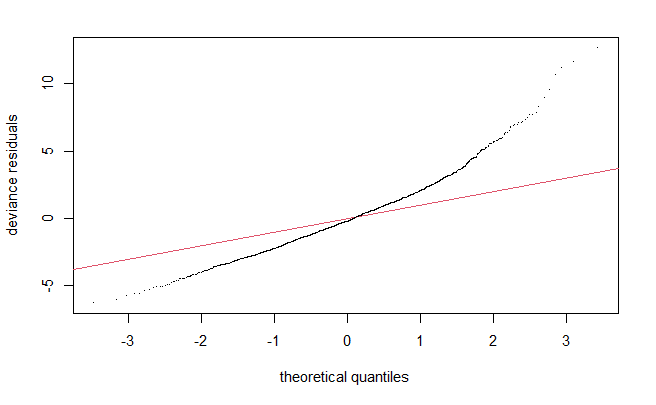
\includegraphics{QQ.png}

}

\caption{QQ Plot}

\end{figure}

Our QQ-plot suggest that the quantiles in our data our not similar to
the line as it deviates from the line in nearly all the values, showing
a very flawed fit. As this suggests that our current model doesn't fit
the data correctly and required an extension to our model as the Poisson
GAM is not accounted for enough deviance as seen in the residuals.

Since the model is not accounting for enough of the variance we will
check if there is a significant difference between the variance and the
mean. In this analyses we will use the Pearson estimate for the
dispersion parameter, this method allow us to estimate the amount of
extra variability, or over-dispersion in count data and therefore
analyse if the Poisson distribution assumption of equal mean and
variance holds.

\hypertarget{model-evaluation}{%
\subsection{Model Evaluation:}\label{model-evaluation}}

\begin{figure}

{\centering \includegraphics{Dispersion.png}

}

\caption{Dispersion Parameter}

\end{figure}

As we can see from the dispersion parameter should be 1 for the
assumption of equal mean and variance to hold true, so it seems that
there is substantial over-dispersion in the Poisson GAM. This violates
one of the Poisson assumptions that the mean and variance are equal
therefore we will have to extend the model from e GAM Poisson to a
Negative Binomial GAM

As we can see from the residual versus predictor plot, the values seem
to be randomly scattered with no clear trend but with some distance from
the zero line. As such we can determine that this scatter is due to
random errors and not a unacounted patern in the model.

\begin{figure}

{\centering 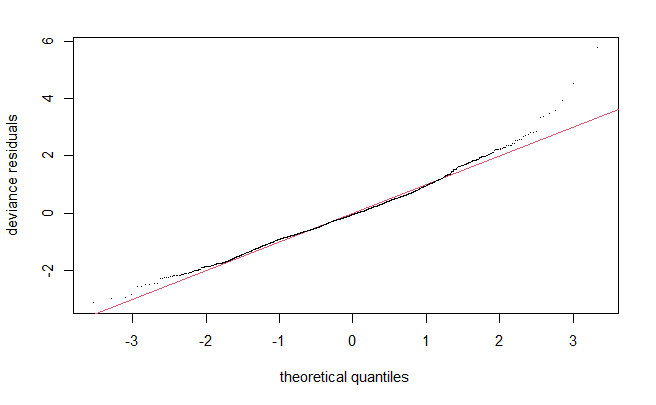
\includegraphics{QQNB.png}

}

\caption{QQ - Negative Binomial}

\end{figure}

The QQ-plot looks much better for the Negative Binomial model. The
majority of points lie either on top of very near the y=x line, except
for a few towards the extremes. This indicates our assumption about the
true distribution of the data is a lot more safe than it was before.

\hypertarget{todo-add-thre-residual-sum-here}{%
\subsection{TODO add thre residual sum
here}\label{todo-add-thre-residual-sum-here}}

sum(residuals(nb\_model, type = ``pearson'')\^{}2) /
df.residual(nb\_model)

The dispersion parameter is very close to 1, unlike for the Poisson
model, meaning that the model that can account for most of the
over-dispersion in the data. As such a dispersion parameter value close
to 1 can be interpreted as the model is a good fit for the data due to
the model adequately capture the variability of the the response
variable.

\hypertarget{results-and-interpretation}{%
\subsection{Results and
Interpretation:}\label{results-and-interpretation}}

\hypertarget{conclusion}{%
\subsection{Conclusion:}\label{conclusion}}

\hypertarget{apendix}{%
\subsection{Apendix}\label{apendix}}

\begin{Shaded}
\begin{Highlighting}[]
\DocumentationTok{\#\# PLotting map of cases}
\FunctionTok{plot.map}\NormalTok{(TBdata}\SpecialCharTok{$}\NormalTok{TB[TBdata}\SpecialCharTok{$}\NormalTok{Year }\SpecialCharTok{==} \DecValTok{2014}\NormalTok{], }\AttributeTok{n.levels =} \DecValTok{7}\NormalTok{, }\AttributeTok{main =} \StringTok{"TB counts for 2014"}\NormalTok{)}
\end{Highlighting}
\end{Shaded}

\begin{figure}[H]

{\centering 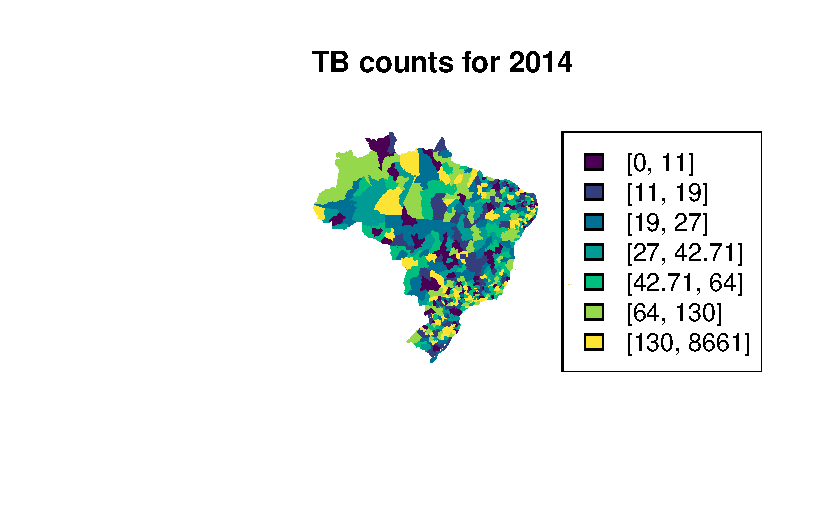
\includegraphics{Group34Coursework_files/figure-pdf/unnamed-chunk-2-1.pdf}

}

\end{figure}

\hypertarget{exploratory-analyses}{%
\subsection{Exploratory analyses}\label{exploratory-analyses}}

\begin{Shaded}
\begin{Highlighting}[]
\FunctionTok{plot\_histogram}\NormalTok{(TBdata)}
\end{Highlighting}
\end{Shaded}

\begin{figure}[H]

{\centering 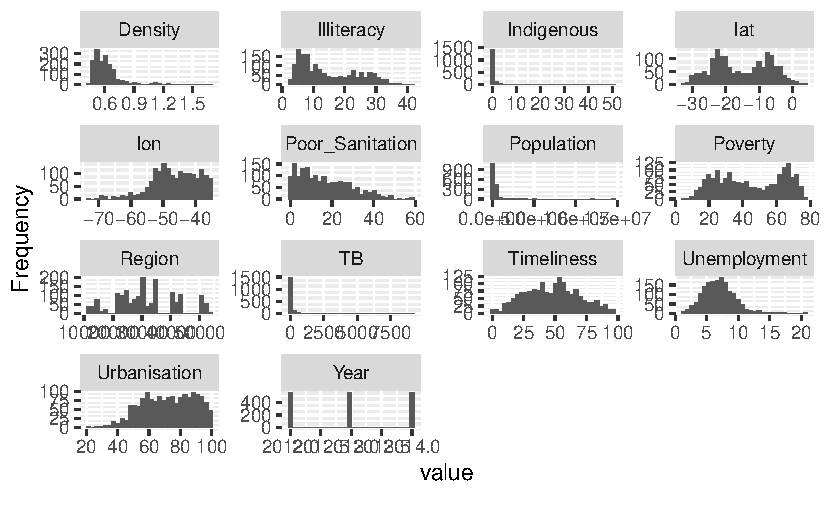
\includegraphics{Group34Coursework_files/figure-pdf/unnamed-chunk-5-1.pdf}

}

\end{figure}

//TODO talk about the histograms and relevant distributions we can
observe

Now investigating the correlation matrix of the numerical variables

\begin{Shaded}
\begin{Highlighting}[]
\FunctionTok{plot\_correlation}\NormalTok{(TBdata)}
\end{Highlighting}
\end{Shaded}

\begin{figure}[H]

{\centering 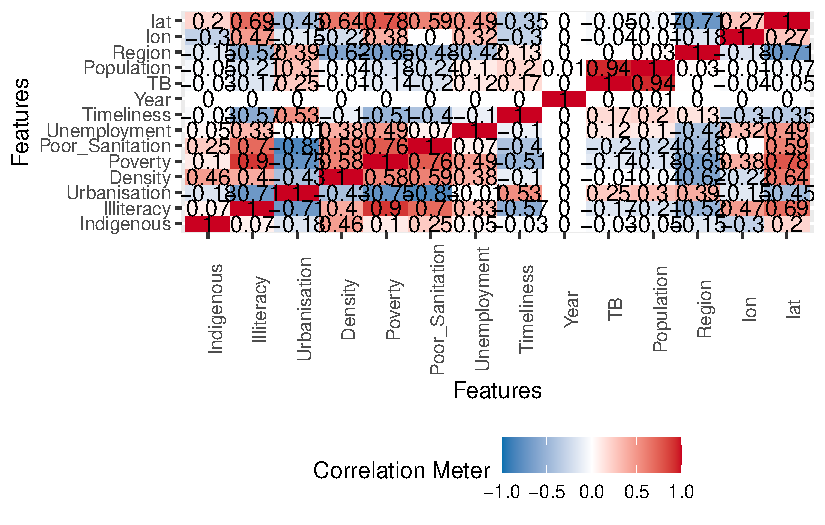
\includegraphics{Group34Coursework_files/figure-pdf/unnamed-chunk-6-1.pdf}

}

\end{figure}

As we can see from the matrix, the variable that is the most correlated
from TB is the population, with illiteracy, poor sanitation and poverty
having a negative correlation with TB.

\hypertarget{poisson-definition}{%
\subsection{Poisson definition}\label{poisson-definition}}

As the data is count data we will first fit a Poisson module since this
distribution is a good fit for the nature of the data

\begin{Shaded}
\begin{Highlighting}[]
\NormalTok{poisson\_model }\OtherTok{\textless{}{-}} \FunctionTok{gam}\NormalTok{(TB }\SpecialCharTok{\textasciitilde{}} \FunctionTok{offset}\NormalTok{(}\FunctionTok{log}\NormalTok{(Population)) }\SpecialCharTok{+} \FunctionTok{s}\NormalTok{(Indigenous, }\AttributeTok{k =} \DecValTok{20}\NormalTok{) }\SpecialCharTok{+} \FunctionTok{s}\NormalTok{(Illiteracy , }\AttributeTok{k =} \DecValTok{20}\NormalTok{) }\SpecialCharTok{+} \FunctionTok{s}\NormalTok{(Urbanisation, }\AttributeTok{k =} \DecValTok{20}\NormalTok{) }\SpecialCharTok{+} \FunctionTok{s}\NormalTok{(Density, }\AttributeTok{k =} \DecValTok{20}\NormalTok{) }\SpecialCharTok{+} \FunctionTok{s}\NormalTok{(Poverty, }\AttributeTok{k =} \DecValTok{20}\NormalTok{) }\SpecialCharTok{+} \FunctionTok{s}\NormalTok{(Poor\_Sanitation, }\AttributeTok{k =} \DecValTok{20}\NormalTok{) }\SpecialCharTok{+} \FunctionTok{s}\NormalTok{(Unemployment, }\AttributeTok{k =} \DecValTok{20}\NormalTok{) }\SpecialCharTok{+} \FunctionTok{s}\NormalTok{(Timeliness, }\AttributeTok{k =} \DecValTok{20}\NormalTok{) }\SpecialCharTok{+} \FunctionTok{s}\NormalTok{(lat, }\AttributeTok{k =} \DecValTok{30}\NormalTok{) }\SpecialCharTok{+} \FunctionTok{s}\NormalTok{(lon, }\AttributeTok{k =} \DecValTok{30}\NormalTok{) }\SpecialCharTok{+} \FunctionTok{s}\NormalTok{(Year, }\AttributeTok{k =} \DecValTok{3}\NormalTok{) }\SpecialCharTok{+} \FunctionTok{ti}\NormalTok{(lon, lat, Year, }\AttributeTok{k =} \DecValTok{3}\NormalTok{), }\AttributeTok{family =}\NormalTok{ poisson, }\AttributeTok{data =}\NormalTok{ TBdata, }\AttributeTok{method =} \StringTok{\textquotesingle{}REML\textquotesingle{}}\NormalTok{)}
\FunctionTok{summary}\NormalTok{(poisson\_model)}
\end{Highlighting}
\end{Shaded}

\begin{verbatim}

Family: poisson 
Link function: log 

Formula:
TB ~ offset(log(Population)) + s(Indigenous, k = 20) + s(Illiteracy, 
    k = 20) + s(Urbanisation, k = 20) + s(Density, k = 20) + 
    s(Poverty, k = 20) + s(Poor_Sanitation, k = 20) + s(Unemployment, 
    k = 20) + s(Timeliness, k = 20) + s(lat, k = 30) + s(lon, 
    k = 30) + s(Year, k = 3) + ti(lon, lat, Year, k = 3)

Parametric coefficients:
             Estimate Std. Error z value Pr(>|z|)    
(Intercept) -8.480233   0.004557   -1861   <2e-16 ***
---
Signif. codes:  0 '***' 0.001 '**' 0.01 '*' 0.05 '.' 0.1 ' ' 1

Approximate significance of smooth terms:
                      edf Ref.df  Chi.sq p-value    
s(Indigenous)      18.443 18.925  649.18 < 2e-16 ***
s(Illiteracy)      18.262 18.907  439.58 < 2e-16 ***
s(Urbanisation)    18.888 18.991  741.26 < 2e-16 ***
s(Density)         17.130 17.913  525.38 < 2e-16 ***
s(Poverty)         18.502 18.917 1176.23 < 2e-16 ***
s(Poor_Sanitation) 17.517 18.656  858.89 < 2e-16 ***
s(Unemployment)    18.475 18.944 1450.40 < 2e-16 ***
s(Timeliness)      18.159 18.868  911.93 < 2e-16 ***
s(lat)             28.310 28.939 2406.85 < 2e-16 ***
s(lon)             28.447 28.951 2601.82 < 2e-16 ***
s(Year)             1.847  1.962   46.82 < 2e-16 ***
ti(lon,lat,Year)    3.913  5.017   16.61 0.00535 ** 
---
Signif. codes:  0 '***' 0.001 '**' 0.01 '*' 0.05 '.' 0.1 ' ' 1

R-sq.(adj) =  0.997   Deviance explained = 87.9%
-REML = 9825.5  Scale est. = 1         n = 1671
\end{verbatim}

\begin{Shaded}
\begin{Highlighting}[]
\FunctionTok{gam.check}\NormalTok{(poisson\_model)}
\end{Highlighting}
\end{Shaded}

\begin{Shaded}
\begin{Highlighting}[]
\CommentTok{\#Akaike Information Criterion:}
\NormalTok{poisson\_model}\SpecialCharTok{$}\NormalTok{aic}
\end{Highlighting}
\end{Shaded}

\begin{verbatim}
[1] 18585.52
\end{verbatim}

\begin{Shaded}
\begin{Highlighting}[]
\FunctionTok{plot}\NormalTok{(poisson\_model, }\AttributeTok{shade=}\NormalTok{T, }\AttributeTok{rug =} \ConstantTok{TRUE}\NormalTok{, }\AttributeTok{residuals =} \ConstantTok{TRUE}\NormalTok{,}
\AttributeTok{pch =} \DecValTok{1}\NormalTok{, }\AttributeTok{cex =} \FloatTok{0.5}\NormalTok{)}
\end{Highlighting}
\end{Shaded}

\begin{figure}[H]

{\centering 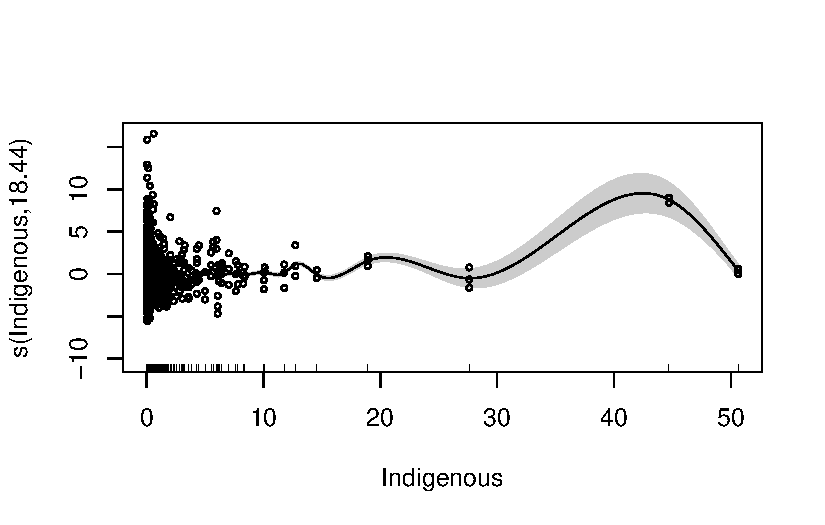
\includegraphics{Group34Coursework_files/figure-pdf/unnamed-chunk-9-1.pdf}

}

\end{figure}

\begin{figure}[H]

{\centering 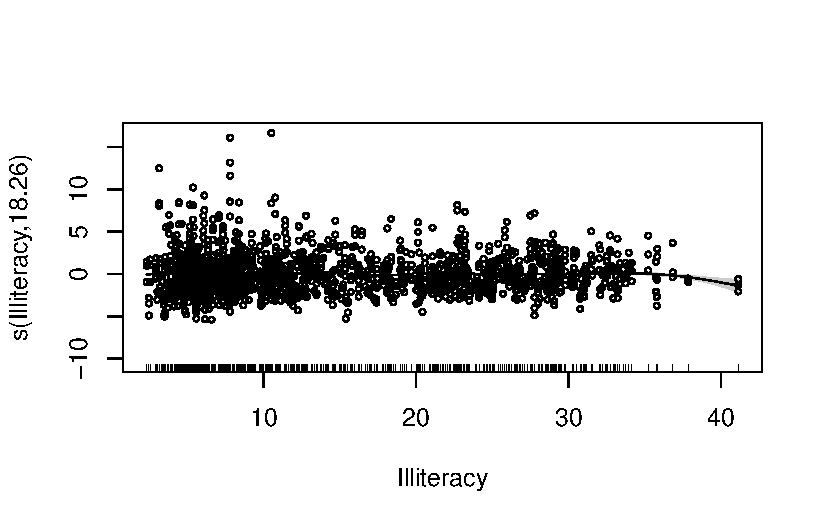
\includegraphics{Group34Coursework_files/figure-pdf/unnamed-chunk-9-2.pdf}

}

\end{figure}

\begin{figure}[H]

{\centering 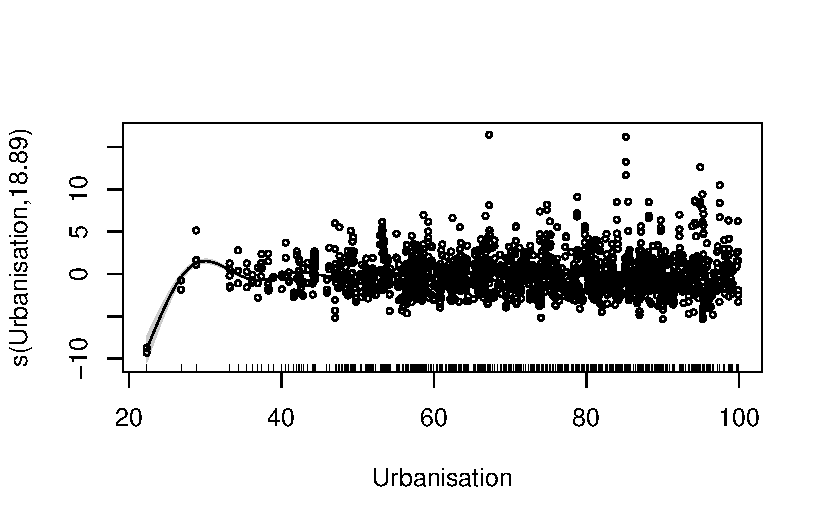
\includegraphics{Group34Coursework_files/figure-pdf/unnamed-chunk-9-3.pdf}

}

\end{figure}

\begin{figure}[H]

{\centering 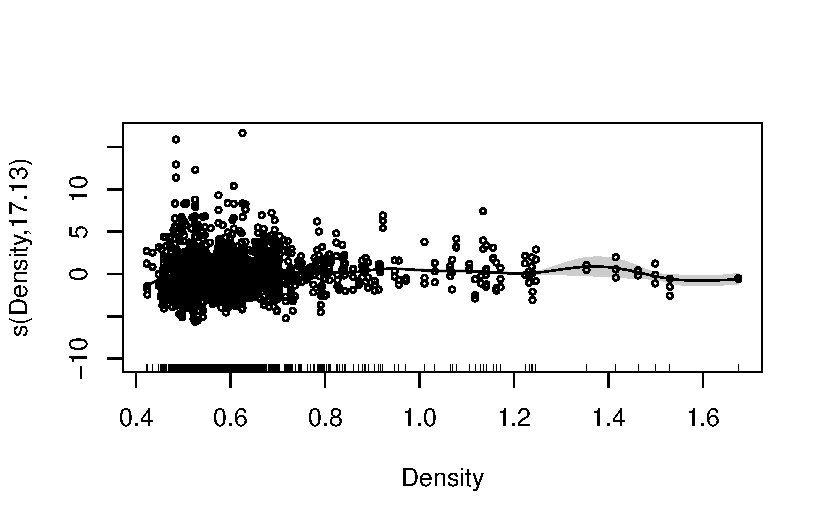
\includegraphics{Group34Coursework_files/figure-pdf/unnamed-chunk-9-4.pdf}

}

\end{figure}

\begin{figure}[H]

{\centering 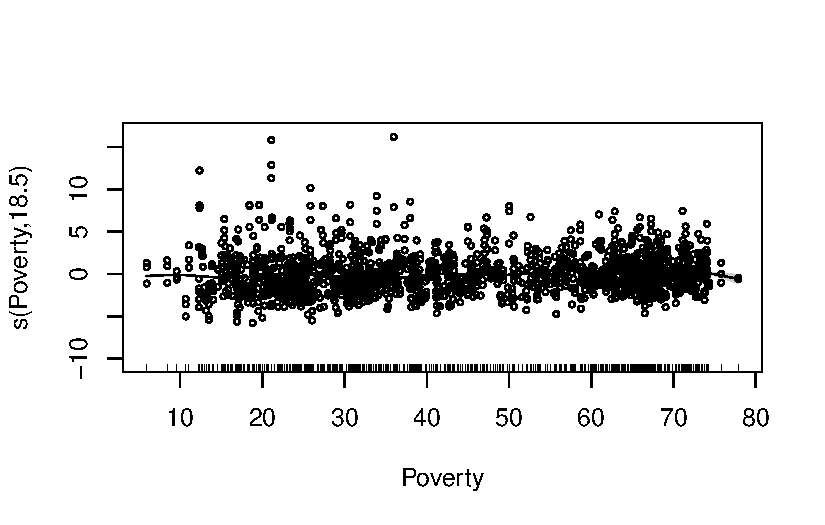
\includegraphics{Group34Coursework_files/figure-pdf/unnamed-chunk-9-5.pdf}

}

\end{figure}

\begin{figure}[H]

{\centering 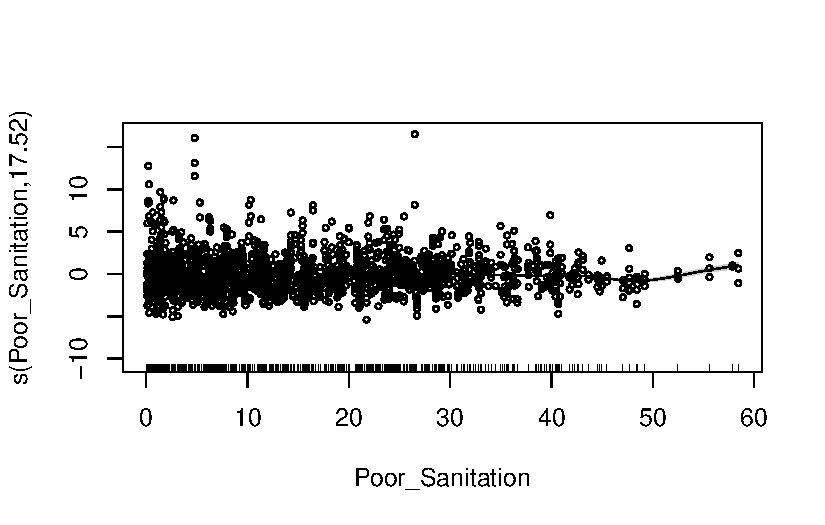
\includegraphics{Group34Coursework_files/figure-pdf/unnamed-chunk-9-6.pdf}

}

\end{figure}

\begin{figure}[H]

{\centering 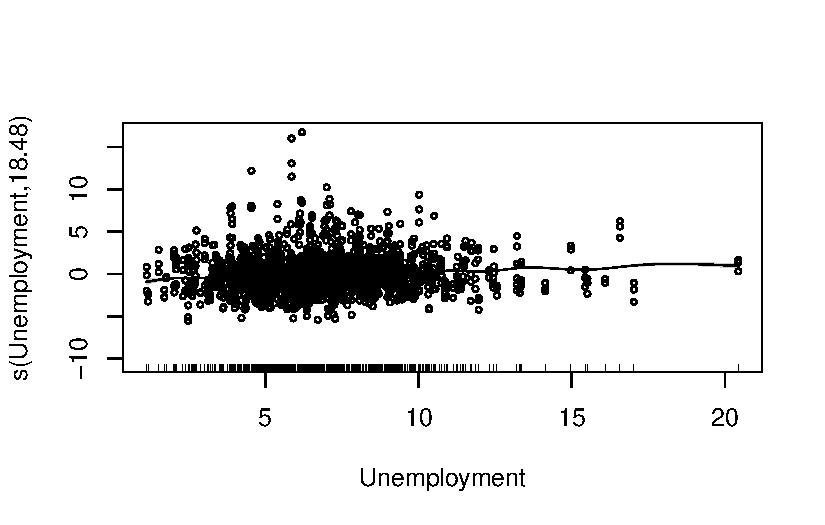
\includegraphics{Group34Coursework_files/figure-pdf/unnamed-chunk-9-7.pdf}

}

\end{figure}

\begin{figure}[H]

{\centering 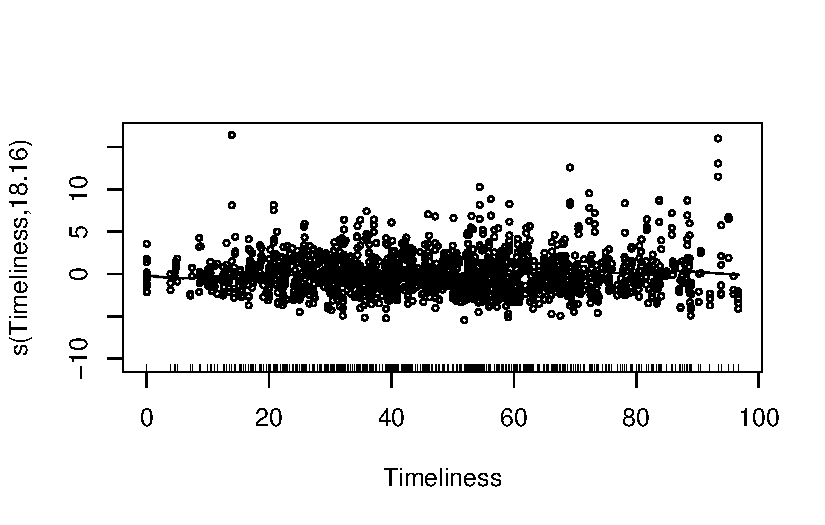
\includegraphics{Group34Coursework_files/figure-pdf/unnamed-chunk-9-8.pdf}

}

\end{figure}

\begin{figure}[H]

{\centering 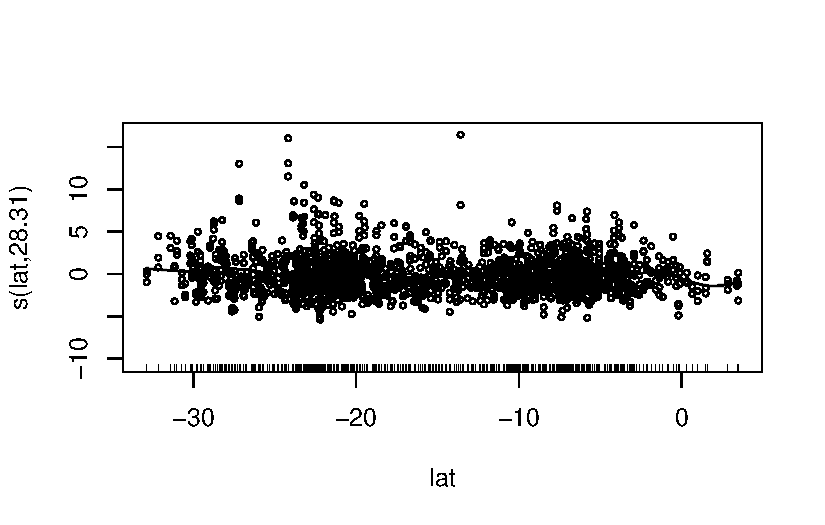
\includegraphics{Group34Coursework_files/figure-pdf/unnamed-chunk-9-9.pdf}

}

\end{figure}

\begin{figure}[H]

{\centering 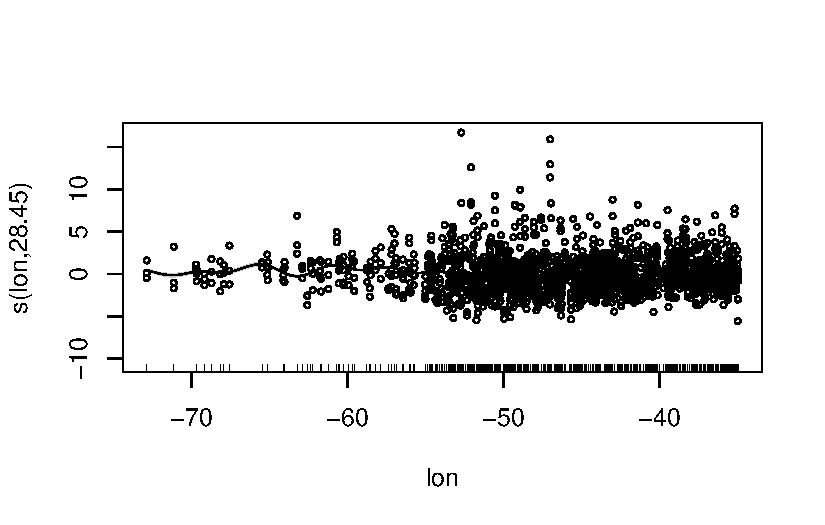
\includegraphics{Group34Coursework_files/figure-pdf/unnamed-chunk-9-10.pdf}

}

\end{figure}

\begin{figure}[H]

{\centering 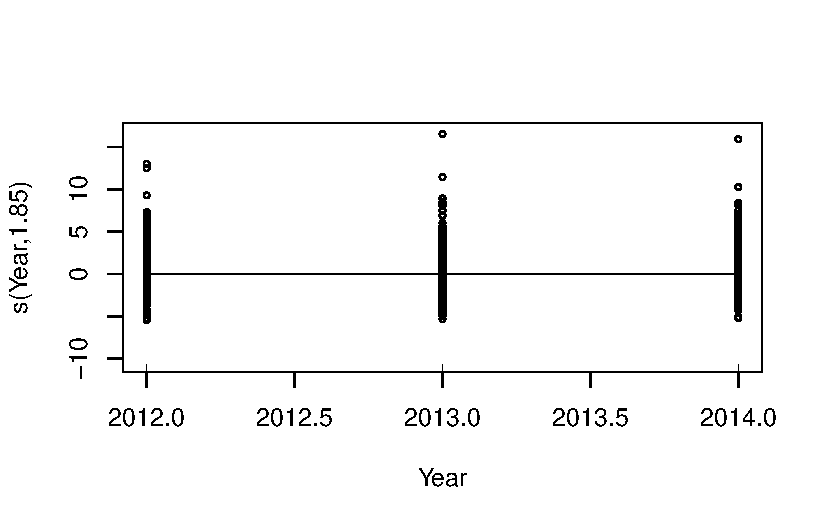
\includegraphics{Group34Coursework_files/figure-pdf/unnamed-chunk-9-11.pdf}

}

\end{figure}

\begin{figure}[H]

{\centering 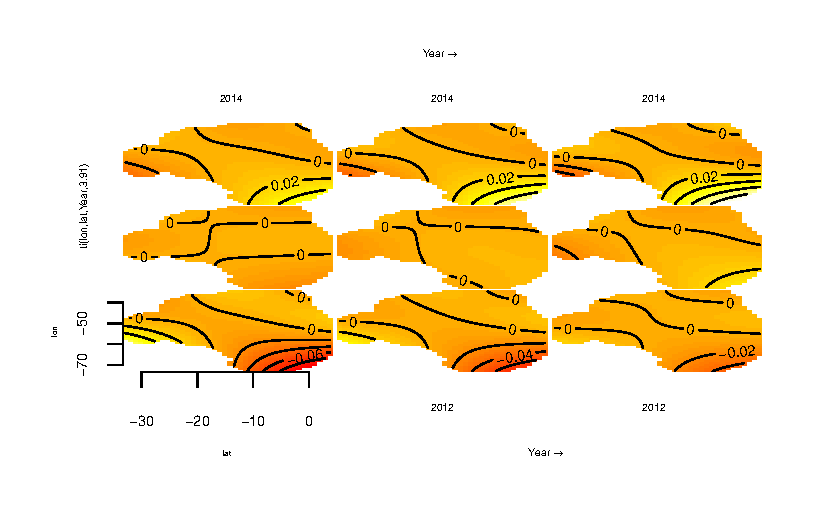
\includegraphics{Group34Coursework_files/figure-pdf/unnamed-chunk-9-12.pdf}

}

\end{figure}

\begin{Shaded}
\begin{Highlighting}[]
\CommentTok{\#Lets check our model residuals:}
\FunctionTok{qq.gam}\NormalTok{(poisson\_model)}
\end{Highlighting}
\end{Shaded}

\begin{figure}[H]

{\centering 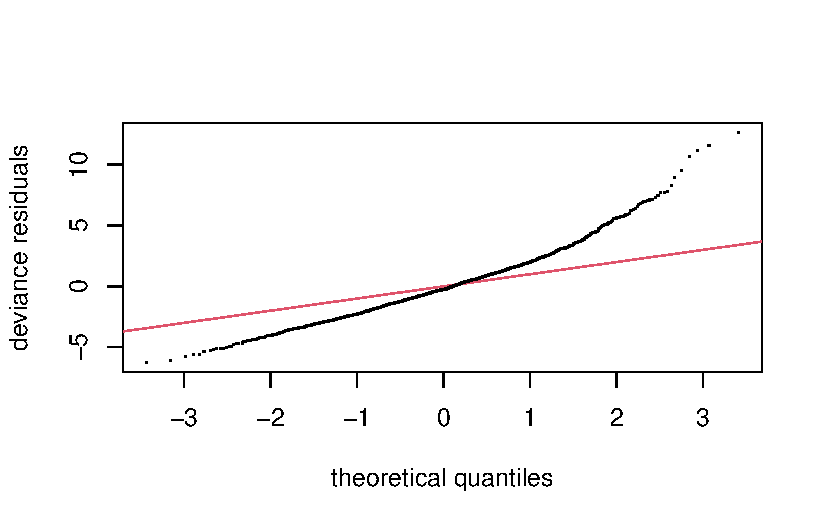
\includegraphics{Group34Coursework_files/figure-pdf/unnamed-chunk-9-13.pdf}

}

\end{figure}

Our QQ-plot suggest that the quantiles in our data our not similar to
the line as it deviates from the line in nearly all the values, showing
a very flawed fit. As this suggests that our current model doesn't fit
the data correctly and required an extension to our model as the Poisson
GAM is not accounted for enough deviance as seen in the residuals.

Since the model is not accounting for enough of the variance we will
check if there is a significant difference between the variance and the
mean. In this analyses we will use the Pearson estimate for the
dispersion parameter, this method allow us to estimate the amount of
extra variability, or over-dispersion in count data and therefore
analyse if the Poisson distribution assumption of equal mean and
variance holds.

\begin{Shaded}
\begin{Highlighting}[]
\CommentTok{\#Calculating Pearson estimate for dispersion parameter using Pearson residuals:}
\FunctionTok{sum}\NormalTok{(}\FunctionTok{residuals}\NormalTok{(poisson\_model, }\AttributeTok{type =} \StringTok{"pearson"}\NormalTok{)}\SpecialCharTok{\^{}}\DecValTok{2}\NormalTok{) }\SpecialCharTok{/} \FunctionTok{df.residual}\NormalTok{(poisson\_model)}
\end{Highlighting}
\end{Shaded}

\begin{verbatim}
[1] 6.67687
\end{verbatim}

\begin{Shaded}
\begin{Highlighting}[]
\CommentTok{\#The dispersion parameter should be 1, so it seems that there is substantial over{-}dispersion in the Poisson GAM.}
\end{Highlighting}
\end{Shaded}

As we can see from the dispersion parameter should be 1 for the
assumption of equal mean and variance to hold true, so it seems that
there is substantial over-dispersion in the Poisson GAM. This violates
one of the Poisson assumptions that the mean and variance are equal
therefore we will have to extend the model from e GAM Poisson to a
Negative Binomial GAM

\hypertarget{negatice-binomial}{%
\subsection{Negatice binomial}\label{negatice-binomial}}

\begin{Shaded}
\begin{Highlighting}[]
\CommentTok{\#fitting a negative{-}binomial model to our TB data:}
\NormalTok{nb\_model }\OtherTok{\textless{}{-}} \FunctionTok{gam}\NormalTok{(TB }\SpecialCharTok{\textasciitilde{}} \FunctionTok{offset}\NormalTok{(}\FunctionTok{log}\NormalTok{(Population)) }\SpecialCharTok{+} \FunctionTok{s}\NormalTok{(Indigenous, }\AttributeTok{k =} \DecValTok{20}\NormalTok{) }\SpecialCharTok{+} \FunctionTok{s}\NormalTok{(Illiteracy , }\AttributeTok{k =} \DecValTok{20}\NormalTok{) }\SpecialCharTok{+} \FunctionTok{s}\NormalTok{(Urbanisation, }\AttributeTok{k =} \DecValTok{20}\NormalTok{) }\SpecialCharTok{+} \FunctionTok{s}\NormalTok{(Density, }\AttributeTok{k =} \DecValTok{20}\NormalTok{) }\SpecialCharTok{+} \FunctionTok{s}\NormalTok{(Poverty, }\AttributeTok{k =} \DecValTok{20}\NormalTok{) }\SpecialCharTok{+} \FunctionTok{s}\NormalTok{(Poor\_Sanitation, }\AttributeTok{k =} \DecValTok{20}\NormalTok{) }\SpecialCharTok{+} \FunctionTok{s}\NormalTok{(Unemployment, }\AttributeTok{k =} \DecValTok{20}\NormalTok{) }\SpecialCharTok{+} \FunctionTok{s}\NormalTok{(Timeliness, }\AttributeTok{k =} \DecValTok{20}\NormalTok{) }\SpecialCharTok{+} \FunctionTok{s}\NormalTok{(lat, }\AttributeTok{k =} \DecValTok{30}\NormalTok{) }\SpecialCharTok{+} \FunctionTok{s}\NormalTok{(lon, }\AttributeTok{k =} \DecValTok{30}\NormalTok{) }\SpecialCharTok{+} \FunctionTok{s}\NormalTok{(Year, }\AttributeTok{k =} \DecValTok{3}\NormalTok{) }\SpecialCharTok{+} \FunctionTok{ti}\NormalTok{(lon, lat, Year, }\AttributeTok{k =} \DecValTok{3}\NormalTok{), }\FunctionTok{negbin}\NormalTok{(}\AttributeTok{theta =} \DecValTok{9}\NormalTok{, }\AttributeTok{link =} \StringTok{"log"}\NormalTok{), }\AttributeTok{data =}\NormalTok{ TBdata, }\AttributeTok{method =} \StringTok{\textquotesingle{}REML\textquotesingle{}}\NormalTok{)}

\FunctionTok{summary}\NormalTok{(nb\_model)}
\end{Highlighting}
\end{Shaded}

\begin{verbatim}

Family: Negative Binomial(9) 
Link function: log 

Formula:
TB ~ offset(log(Population)) + s(Indigenous, k = 20) + s(Illiteracy, 
    k = 20) + s(Urbanisation, k = 20) + s(Density, k = 20) + 
    s(Poverty, k = 20) + s(Poor_Sanitation, k = 20) + s(Unemployment, 
    k = 20) + s(Timeliness, k = 20) + s(lat, k = 30) + s(lon, 
    k = 30) + s(Year, k = 3) + ti(lon, lat, Year, k = 3)

Parametric coefficients:
             Estimate Std. Error z value Pr(>|z|)    
(Intercept) -8.451092   0.009451  -894.2   <2e-16 ***
---
Signif. codes:  0 '***' 0.001 '**' 0.01 '*' 0.05 '.' 0.1 ' ' 1

Approximate significance of smooth terms:
                      edf Ref.df  Chi.sq  p-value    
s(Indigenous)       2.875  3.451  18.887 0.000643 ***
s(Illiteracy)       4.772  6.034  11.091 0.079313 .  
s(Urbanisation)     6.599  8.228  33.224 8.79e-05 ***
s(Density)          6.942  8.637 103.826  < 2e-16 ***
s(Poverty)          2.028  2.608   1.074 0.652302    
s(Poor_Sanitation)  8.696 10.680  70.808  < 2e-16 ***
s(Unemployment)     5.532  6.935  92.111  < 2e-16 ***
s(Timeliness)       4.764  5.967  79.993  < 2e-16 ***
s(lat)             21.577 25.088 190.344  < 2e-16 ***
s(lon)             19.462 23.059 239.215  < 2e-16 ***
s(Year)             1.400  1.636   1.888 0.207855    
ti(lon,lat,Year)    1.363  1.592   0.819 0.681850    
---
Signif. codes:  0 '***' 0.001 '**' 0.01 '*' 0.05 '.' 0.1 ' ' 1

R-sq.(adj) =  0.883   Deviance explained = 58.1%
-REML = 7113.6  Scale est. = 1         n = 1671
\end{verbatim}

\begin{Shaded}
\begin{Highlighting}[]
\CommentTok{\#Akaike Information Criterion}
\NormalTok{nb\_model}\SpecialCharTok{$}\NormalTok{aic}
\end{Highlighting}
\end{Shaded}

\begin{verbatim}
[1] 14015.77
\end{verbatim}

As we can see from this Akaike Information Criterion(AIC) the Negative
Binomial has a significantly lower value than the previous 18585,52 from
the GAM Poisson, meaning this is already a better fitting model than the
previous one.

Now we will check the residuals to check for any anomalies on our model
prediction

\begin{Shaded}
\begin{Highlighting}[]
\FunctionTok{gam.check}\NormalTok{(nb\_model)}
\end{Highlighting}
\end{Shaded}

\begin{figure}[H]

{\centering 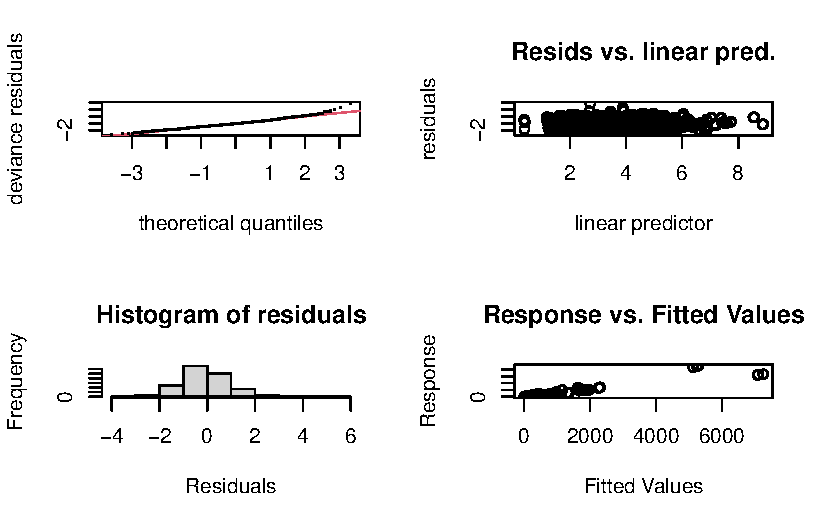
\includegraphics{Group34Coursework_files/figure-pdf/unnamed-chunk-13-1.pdf}

}

\end{figure}

\begin{verbatim}

Method: REML   Optimizer: outer newton
full convergence after 7 iterations.
Gradient range [-0.0008538501,2.782458e-05]
(score 7113.619 & scale 1).
Hessian positive definite, eigenvalue range [0.0001209016,3.084703].
Model rank =  221 / 221 

Basis dimension (k) checking results. Low p-value (k-index<1) may
indicate that k is too low, especially if edf is close to k'.

                      k'   edf k-index p-value    
s(Indigenous)      19.00  2.87    0.54  <2e-16 ***
s(Illiteracy)      19.00  4.77    0.53  <2e-16 ***
s(Urbanisation)    19.00  6.60    0.54  <2e-16 ***
s(Density)         19.00  6.94    0.54  <2e-16 ***
s(Poverty)         19.00  2.03    0.54  <2e-16 ***
s(Poor_Sanitation) 19.00  8.70    0.53  <2e-16 ***
s(Unemployment)    19.00  5.53    0.53  <2e-16 ***
s(Timeliness)      19.00  4.76    0.60  <2e-16 ***
s(lat)             29.00 21.58    0.54  <2e-16 ***
s(lon)             29.00 19.46    0.56  <2e-16 ***
s(Year)             2.00  1.40    0.79  <2e-16 ***
ti(lon,lat,Year)    8.00  1.36    0.94   0.025 *  
---
Signif. codes:  0 '***' 0.001 '**' 0.01 '*' 0.05 '.' 0.1 ' ' 1
\end{verbatim}

As we can see from the residual versus predictor plot, the values seem
to be randomly scattered with no clear trend but with some distance from
the zero line. As such we can determine that this scatter is due to
random errors and not a unacounted patern in the model.

\begin{Shaded}
\begin{Highlighting}[]
\CommentTok{\#checking the model residuals}
\FunctionTok{qq.gam}\NormalTok{(nb\_model)}
\end{Highlighting}
\end{Shaded}

\begin{figure}[H]

{\centering 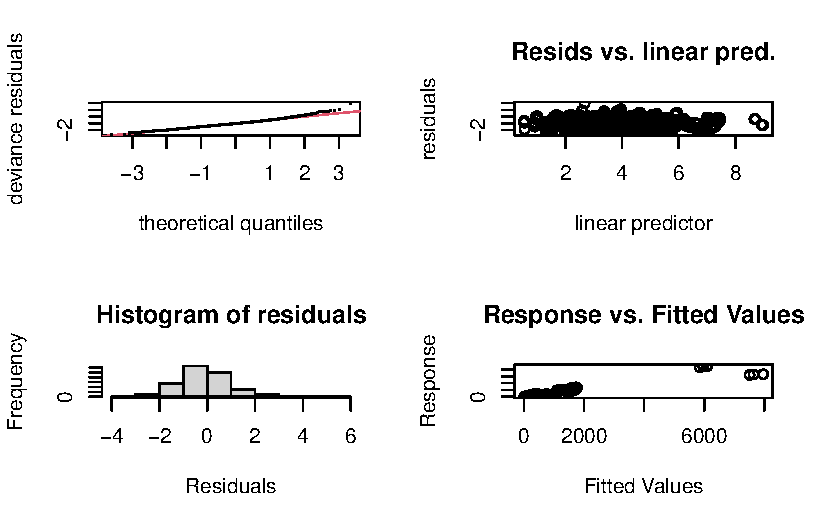
\includegraphics{Group34Coursework_files/figure-pdf/unnamed-chunk-14-1.pdf}

}

\end{figure}

The QQ-plot looks much better for the Negative Binomial model. The
majority of points lie either on top of very near the y=x line, except
for a few towards the extremes. This indicates our assumption about the
true distribution of the data is a lot more safe than it was before.

\begin{Shaded}
\begin{Highlighting}[]
\CommentTok{\#Calculating Pearson estimate for dispersion parameter using Pearson residuals:}
\FunctionTok{sum}\NormalTok{(}\FunctionTok{residuals}\NormalTok{(nb\_model, }\AttributeTok{type =} \StringTok{"pearson"}\NormalTok{)}\SpecialCharTok{\^{}}\DecValTok{2}\NormalTok{) }\SpecialCharTok{/} \FunctionTok{df.residual}\NormalTok{(nb\_model)}
\end{Highlighting}
\end{Shaded}

\begin{verbatim}
[1] 1.190792
\end{verbatim}

The dispersion parameter is very close to 1, unlike for the Poisson
model, meaning that the model that can account for most of the
over-dispersion in the data. As such a dispersion parameter value close
to 1 can be interpreted as the model is a good fit for the data due to
the model adequately capture the variability of the the response
variable.

\hypertarget{again-tidy-up-the-plots-of-the-negative-binomial}{%
\subsection{Again tidy up the plots of the Negative
Binomial}\label{again-tidy-up-the-plots-of-the-negative-binomial}}

\begin{Shaded}
\begin{Highlighting}[]
\FunctionTok{plot}\NormalTok{(nb\_model, }\AttributeTok{shade=}\NormalTok{T, }\AttributeTok{rug =} \ConstantTok{TRUE}\NormalTok{, }\AttributeTok{residuals =} \ConstantTok{TRUE}\NormalTok{,}\AttributeTok{scheme=}\DecValTok{1}\NormalTok{,}
\AttributeTok{pch =} \DecValTok{1}\NormalTok{, }\AttributeTok{cex =} \FloatTok{0.5}\NormalTok{)}
\end{Highlighting}
\end{Shaded}

\begin{figure}[H]

{\centering 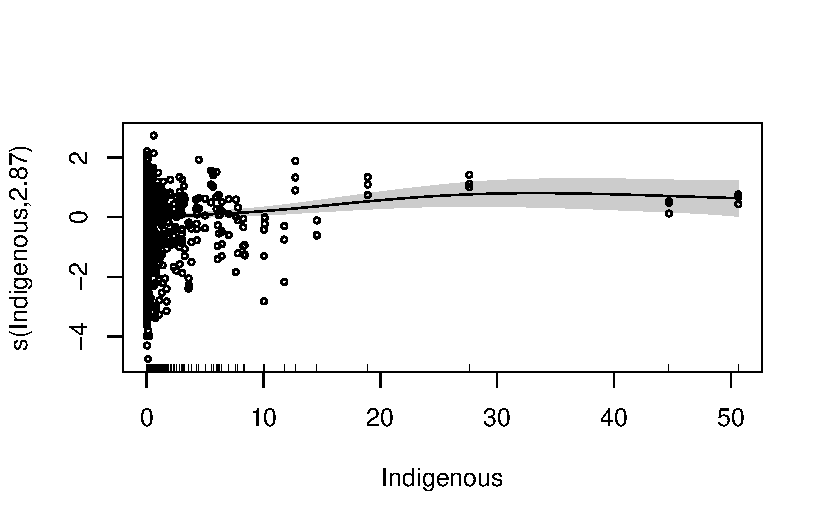
\includegraphics{Group34Coursework_files/figure-pdf/unnamed-chunk-16-1.pdf}

}

\end{figure}

\begin{figure}[H]

{\centering 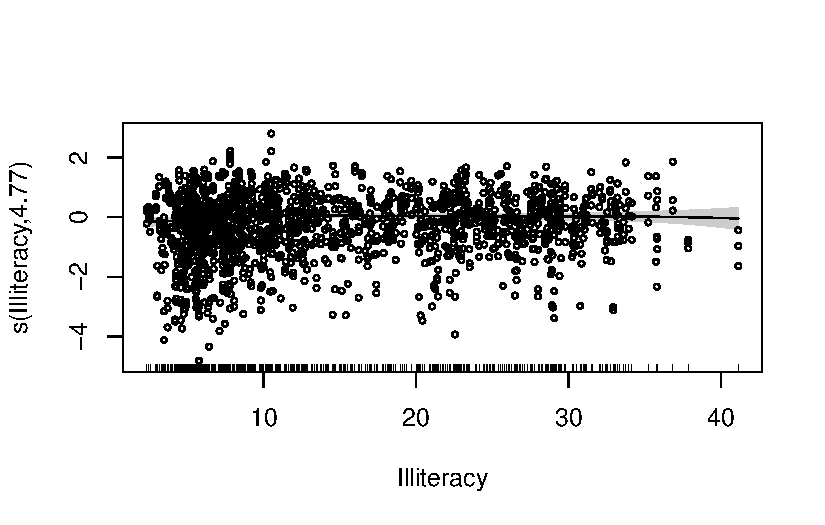
\includegraphics{Group34Coursework_files/figure-pdf/unnamed-chunk-16-2.pdf}

}

\end{figure}

\begin{figure}[H]

{\centering 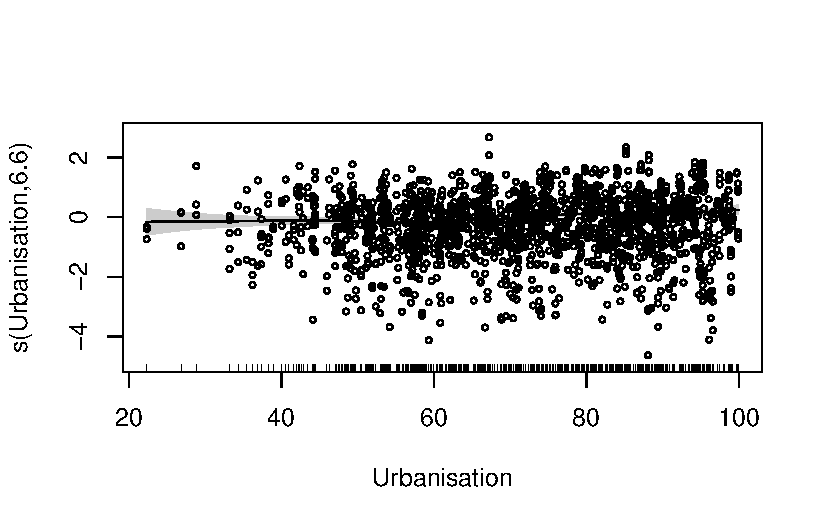
\includegraphics{Group34Coursework_files/figure-pdf/unnamed-chunk-16-3.pdf}

}

\end{figure}

\begin{figure}[H]

{\centering 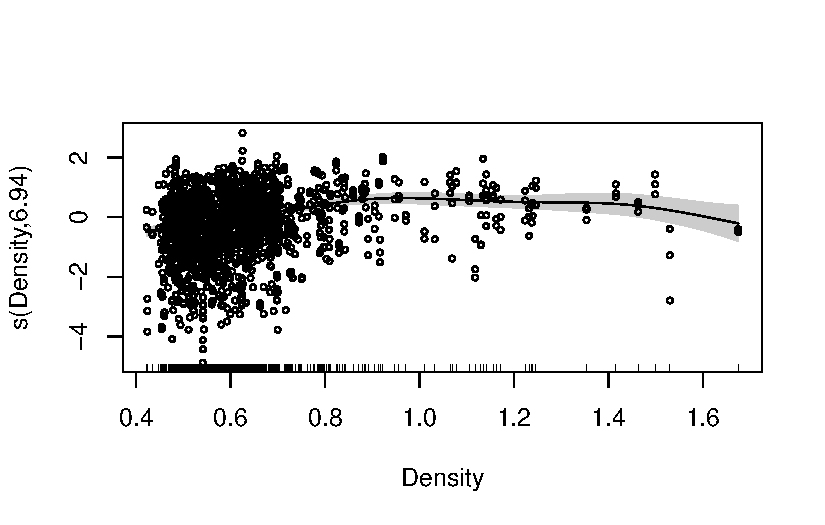
\includegraphics{Group34Coursework_files/figure-pdf/unnamed-chunk-16-4.pdf}

}

\end{figure}

\begin{figure}[H]

{\centering 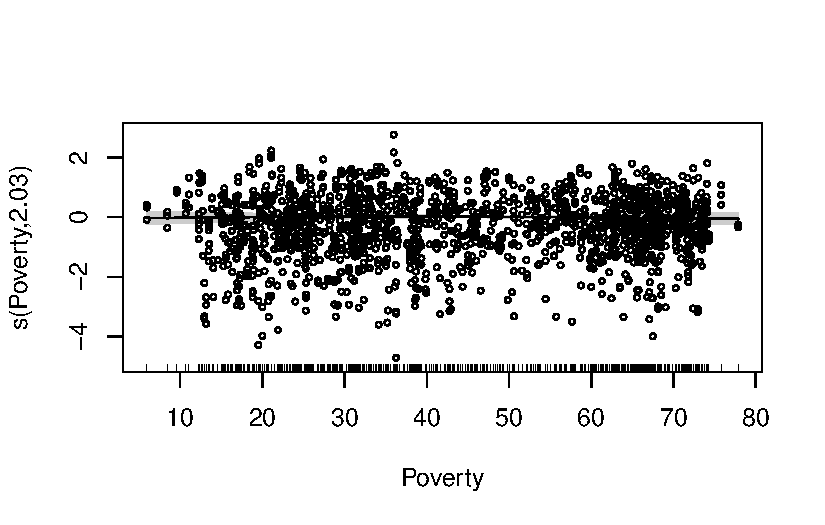
\includegraphics{Group34Coursework_files/figure-pdf/unnamed-chunk-16-5.pdf}

}

\end{figure}

\begin{figure}[H]

{\centering 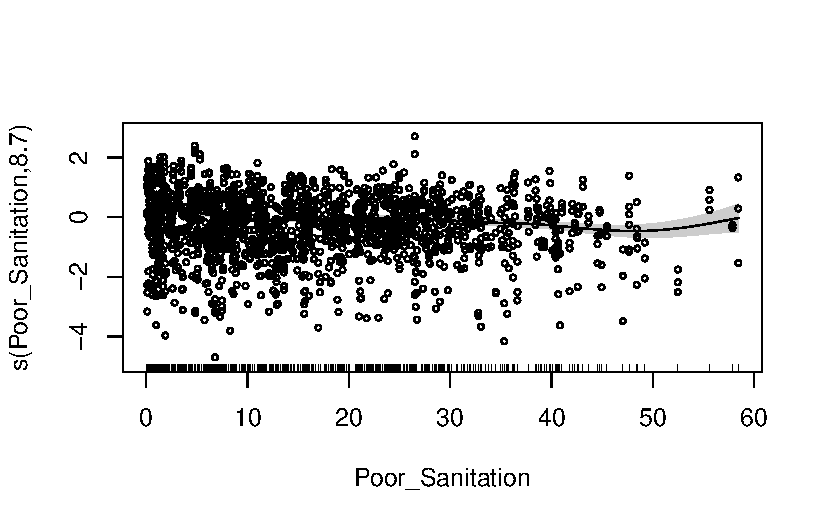
\includegraphics{Group34Coursework_files/figure-pdf/unnamed-chunk-16-6.pdf}

}

\end{figure}

\begin{figure}[H]

{\centering 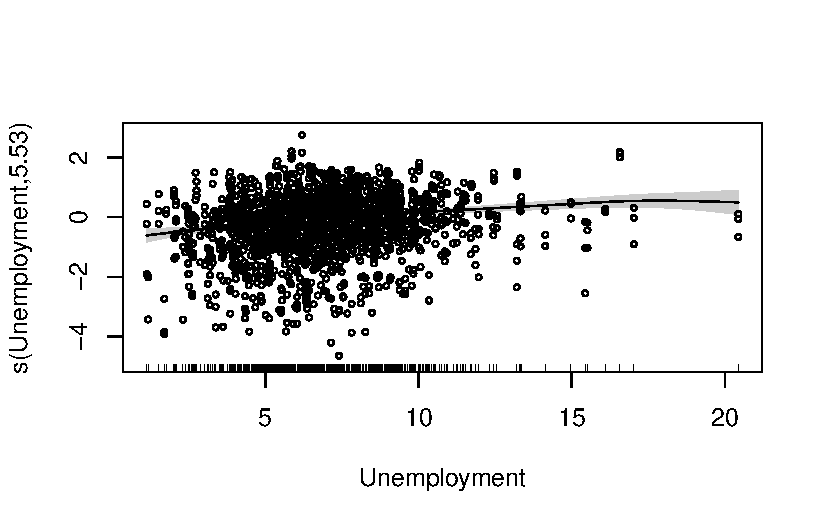
\includegraphics{Group34Coursework_files/figure-pdf/unnamed-chunk-16-7.pdf}

}

\end{figure}

\begin{figure}[H]

{\centering 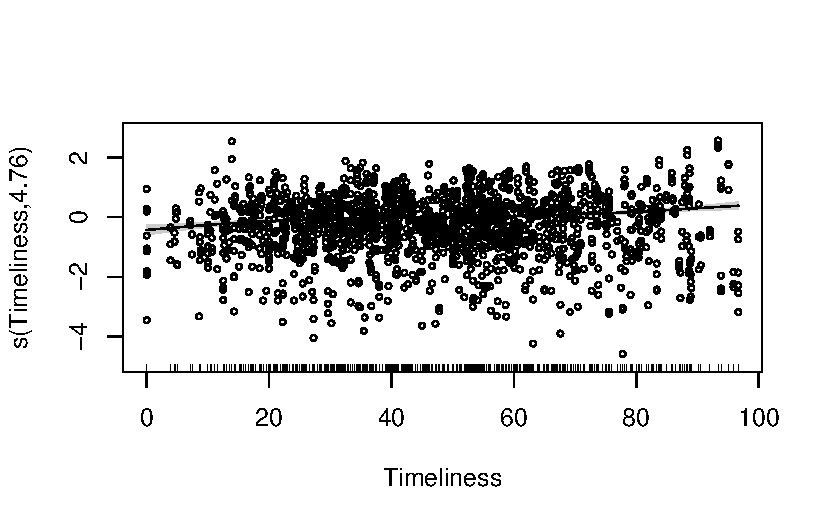
\includegraphics{Group34Coursework_files/figure-pdf/unnamed-chunk-16-8.pdf}

}

\end{figure}

\begin{figure}[H]

{\centering 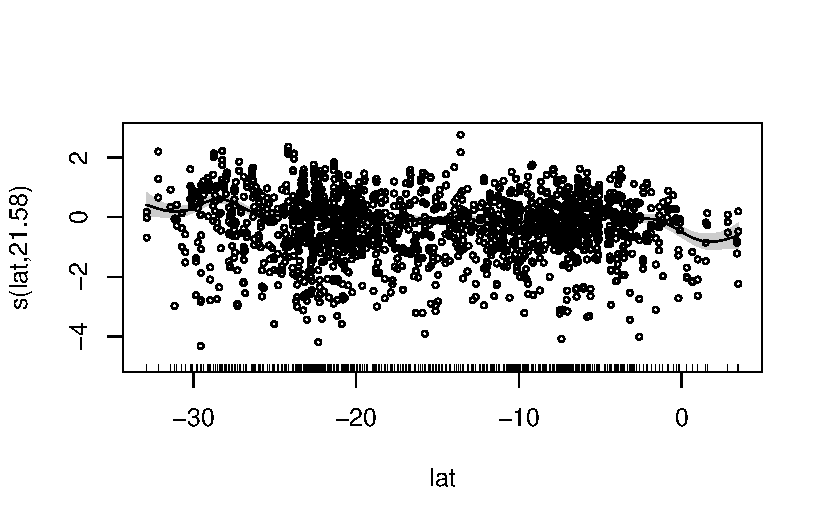
\includegraphics{Group34Coursework_files/figure-pdf/unnamed-chunk-16-9.pdf}

}

\end{figure}

\begin{figure}[H]

{\centering 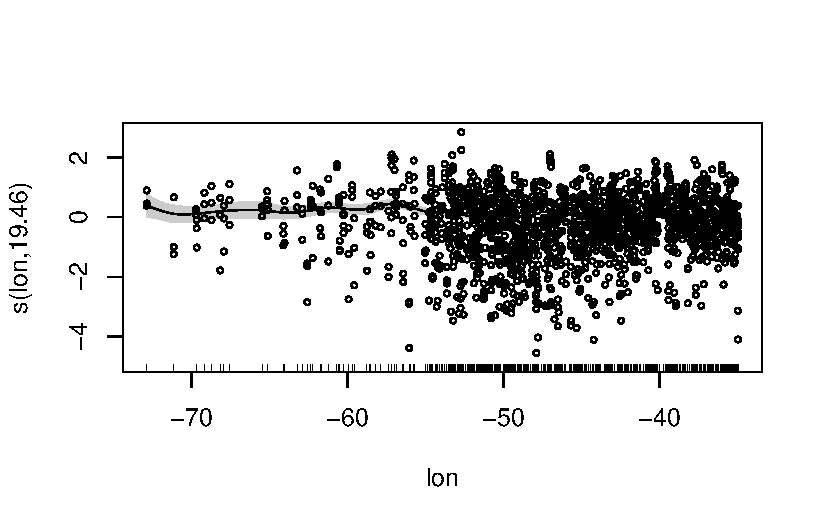
\includegraphics{Group34Coursework_files/figure-pdf/unnamed-chunk-16-10.pdf}

}

\end{figure}

\begin{figure}[H]

{\centering 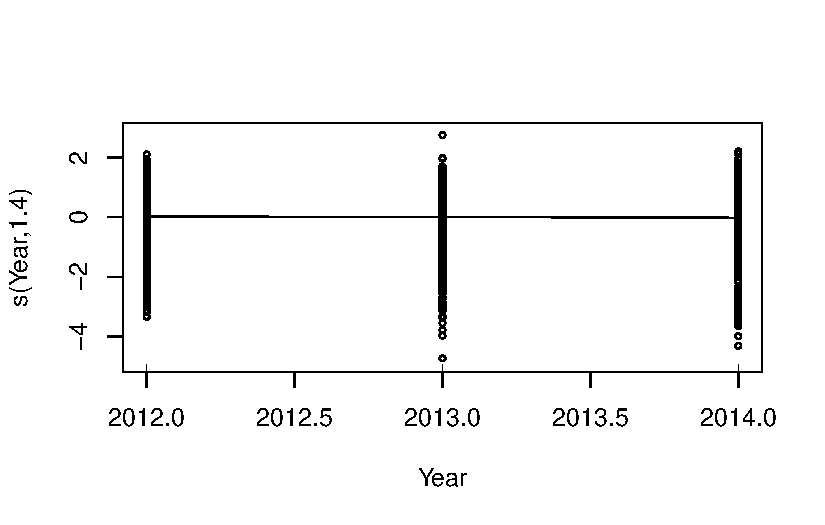
\includegraphics{Group34Coursework_files/figure-pdf/unnamed-chunk-16-11.pdf}

}

\end{figure}

\begin{figure}[H]

{\centering 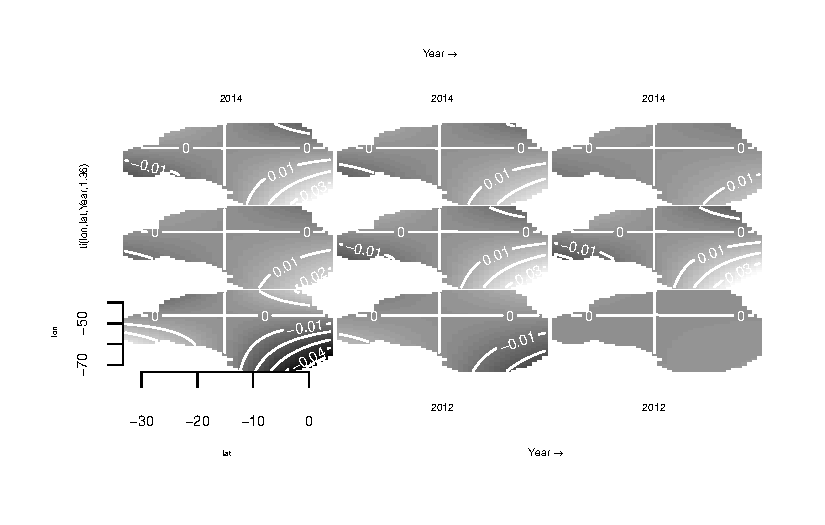
\includegraphics{Group34Coursework_files/figure-pdf/unnamed-chunk-16-12.pdf}

}

\end{figure}

\begin{Shaded}
\begin{Highlighting}[]
\FunctionTok{plot}\NormalTok{(nb\_model, }\AttributeTok{shade =}\NormalTok{ T, }\AttributeTok{rug =} \ConstantTok{TRUE}\NormalTok{, }\AttributeTok{residuals =} \ConstantTok{TRUE}\NormalTok{, }\AttributeTok{scheme =} \DecValTok{2}\NormalTok{, }\AttributeTok{pch =} \DecValTok{1}\NormalTok{,}
    \AttributeTok{cex =} \FloatTok{0.5}\NormalTok{)}
\end{Highlighting}
\end{Shaded}

\begin{figure}[H]

{\centering 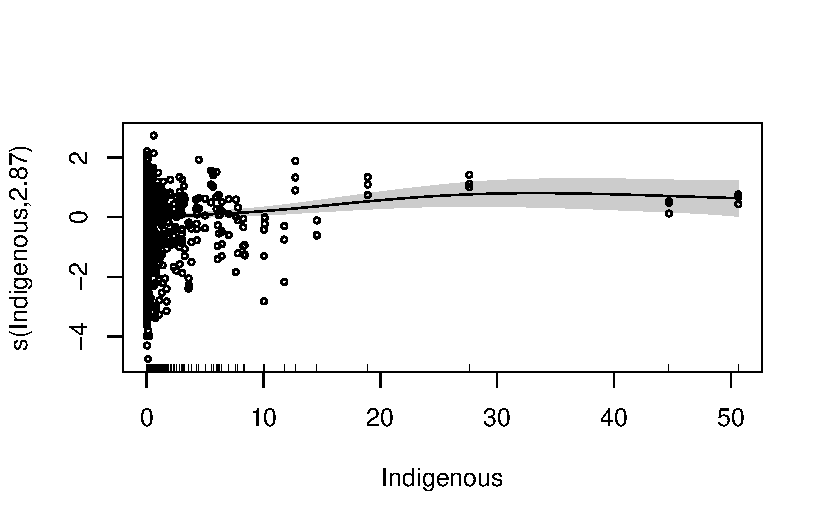
\includegraphics{Group34Coursework_files/figure-pdf/unnamed-chunk-17-1.pdf}

}

\end{figure}

\begin{figure}[H]

{\centering 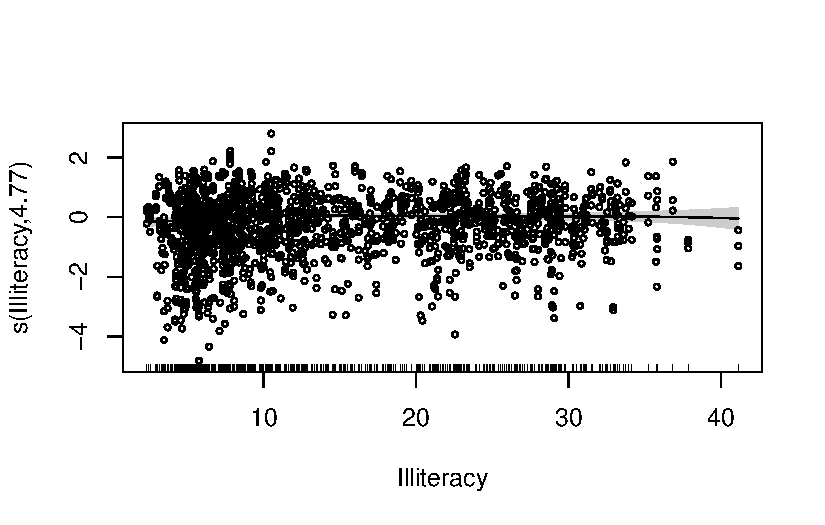
\includegraphics{Group34Coursework_files/figure-pdf/unnamed-chunk-17-2.pdf}

}

\end{figure}

\begin{figure}[H]

{\centering 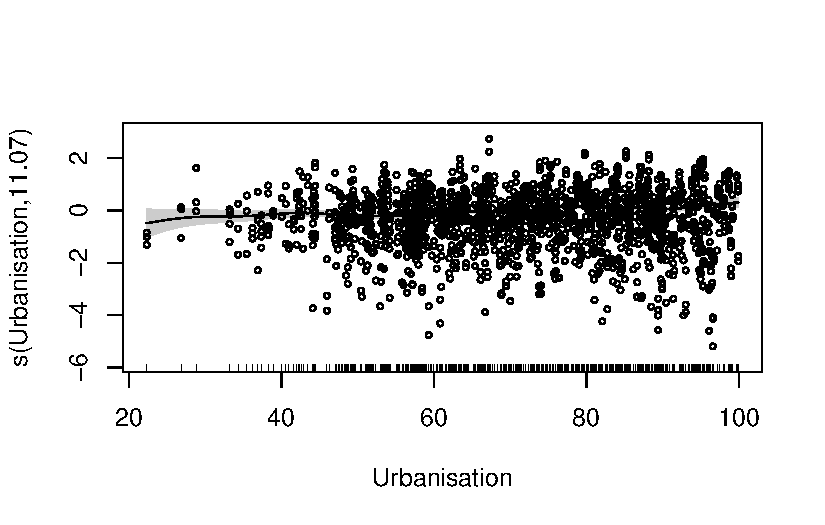
\includegraphics{Group34Coursework_files/figure-pdf/unnamed-chunk-17-3.pdf}

}

\end{figure}

\begin{figure}[H]

{\centering 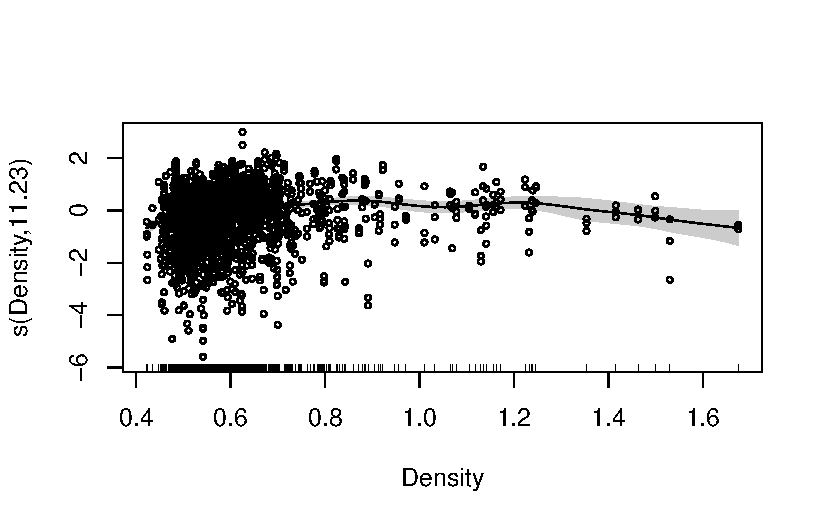
\includegraphics{Group34Coursework_files/figure-pdf/unnamed-chunk-17-4.pdf}

}

\end{figure}

\begin{figure}[H]

{\centering 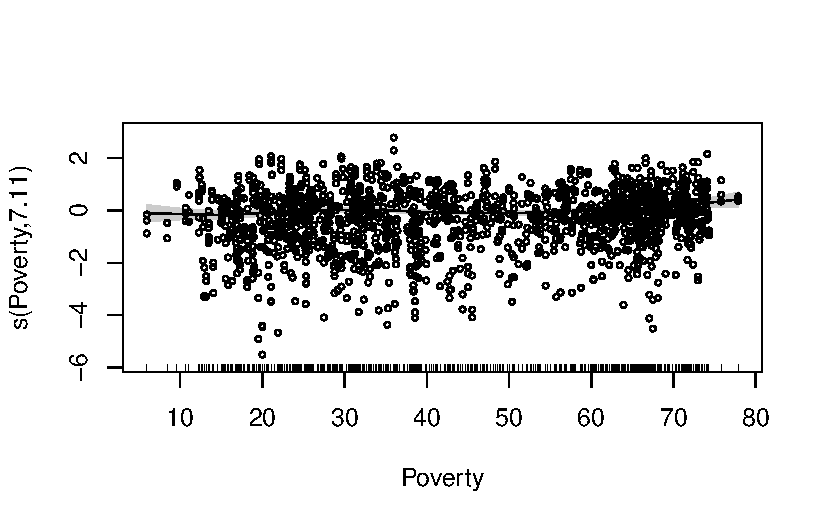
\includegraphics{Group34Coursework_files/figure-pdf/unnamed-chunk-17-5.pdf}

}

\end{figure}

\begin{figure}[H]

{\centering 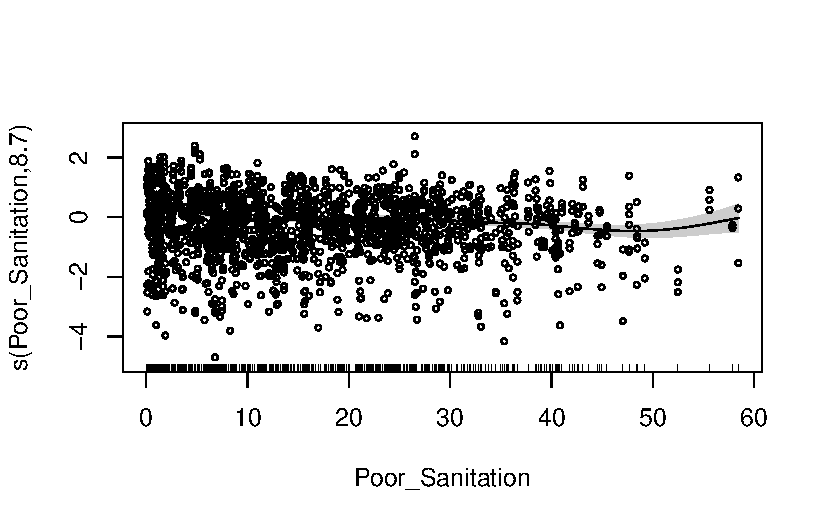
\includegraphics{Group34Coursework_files/figure-pdf/unnamed-chunk-17-6.pdf}

}

\end{figure}

\begin{figure}[H]

{\centering 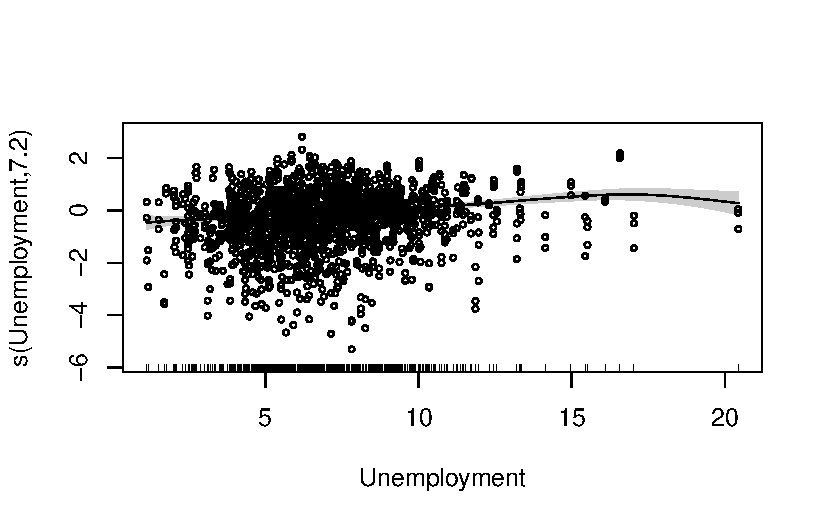
\includegraphics{Group34Coursework_files/figure-pdf/unnamed-chunk-17-7.pdf}

}

\end{figure}

\begin{figure}[H]

{\centering 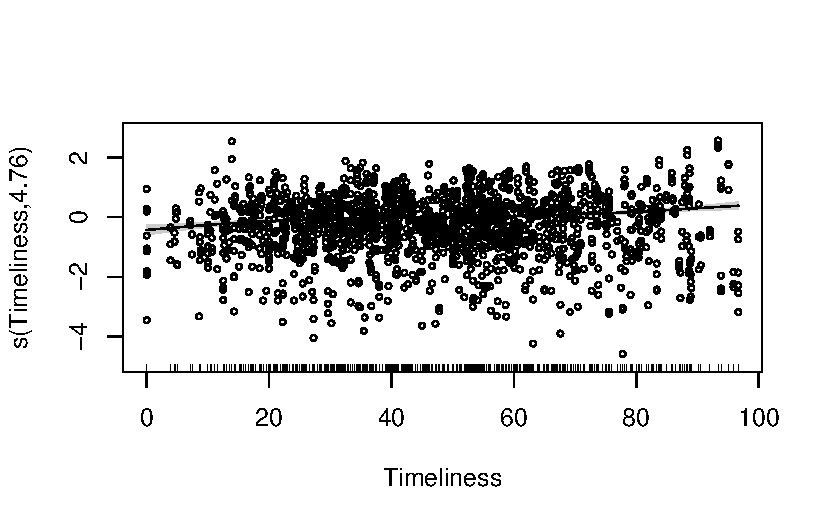
\includegraphics{Group34Coursework_files/figure-pdf/unnamed-chunk-17-8.pdf}

}

\end{figure}

\begin{figure}[H]

{\centering 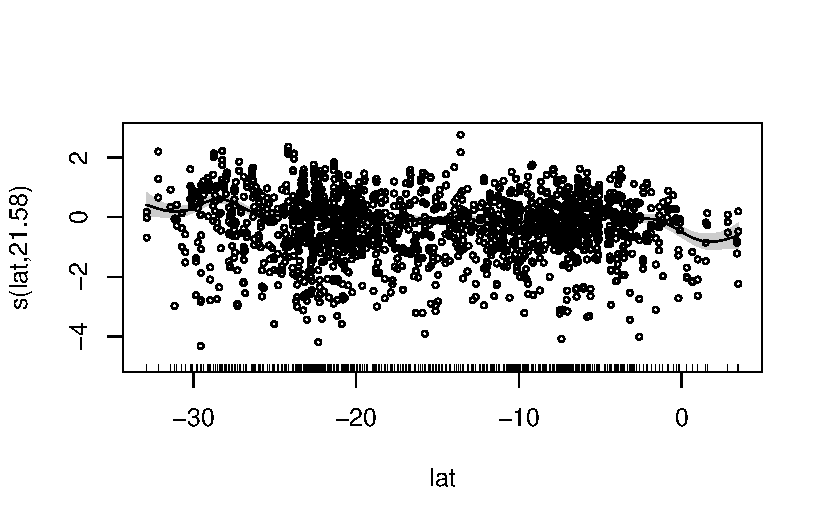
\includegraphics{Group34Coursework_files/figure-pdf/unnamed-chunk-17-9.pdf}

}

\end{figure}

\begin{figure}[H]

{\centering 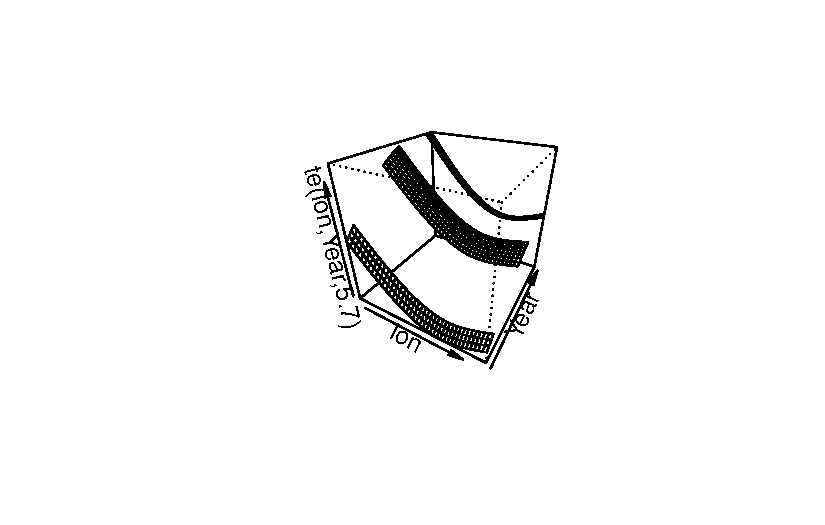
\includegraphics{Group34Coursework_files/figure-pdf/unnamed-chunk-17-10.pdf}

}

\end{figure}

\begin{figure}[H]

{\centering 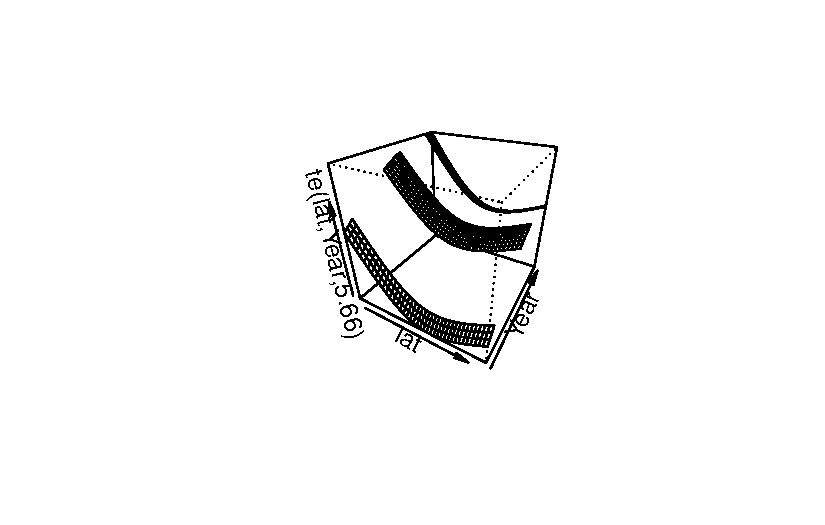
\includegraphics{Group34Coursework_files/figure-pdf/unnamed-chunk-17-11.pdf}

}

\end{figure}

\begin{figure}[H]

{\centering 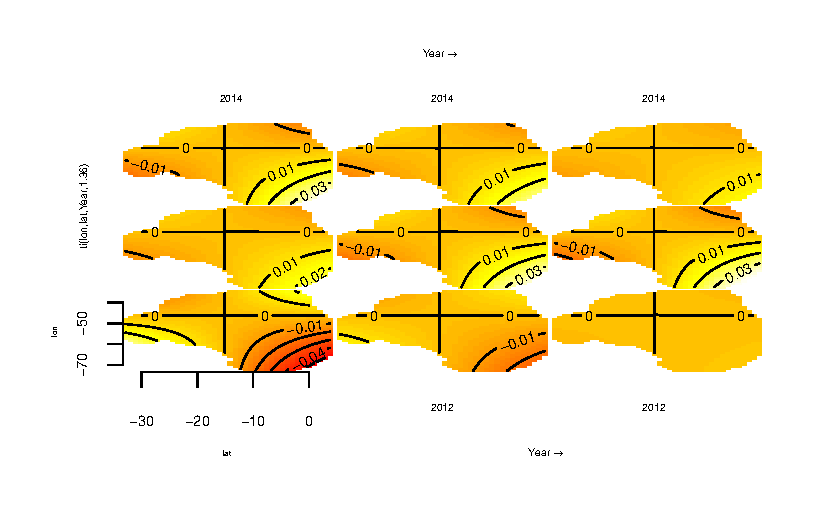
\includegraphics{Group34Coursework_files/figure-pdf/unnamed-chunk-17-12.pdf}

}

\end{figure}

\hypertarget{refs}{}
\begin{CSLReferences}{1}{0}
\leavevmode\vadjust pre{\hypertarget{ref-who_tb_2020}{}}%
\emph{Global Tuberculosis Report 2020}. 2020. Gen{è}ve, Switzerland:
World Health Organization.

\end{CSLReferences}



\end{document}
